% Leakage composition: the 3-bit CLA with its ports and 42 gates, one NAND2 at a = 1, b = 0 zoomed in, the
% terminal currents of its transistors by source (model or Kirchhoff) and whether they enter the gate sum,
% and the adder leakage as the sum of the gate leakages.
% Netlist from scripts/gates.py (NAND2, _nmos, _pmos, CLA_INSTANCES), composition from 07_gates_ml.py
% (balanced_currents, gate_nodes_held_high) and 09_cla_ml.py.
% Build: pdflatex composition.tex && pdfcrop --margins 4 composition.pdf composition.pdf
\documentclass{article}
\usepackage[paperwidth=40cm,paperheight=20cm,margin=1cm]{geometry}
\usepackage[scaled=0.92]{helvet}
\renewcommand{\familydefault}{\sfdefault}
\usepackage[eulergreek]{sansmath}
\usepackage{tikz}
\usetikzlibrary{positioning,calc,arrows.meta,fit,backgrounds}
\pagestyle{empty}

\definecolor{linL}{HTML}{E6F0F8}\definecolor{linD}{HTML}{8EAFCB}
\definecolor{mlpL}{HTML}{E3F1DC}\definecolor{mlpD}{HTML}{98C285}
\definecolor{clsL}{HTML}{FAE3D9}\definecolor{clsD}{HTML}{DFA48A}
\definecolor{newL}{HTML}{FFD563}\definecolor{newD}{HTML}{D79B00}
\definecolor{kclL}{HTML}{BCD7EE}\definecolor{kclD}{HTML}{3D7CB8}
\definecolor{tokL}{HTML}{E8E8E8}\definecolor{tokD}{HTML}{9A9A9A}
\definecolor{arrG}{HTML}{7A7A7A}
\definecolor{emph}{HTML}{E2231A}

\tikzset{
  base/.style={rounded corners=2.5pt, line width=0.55pt, align=center, font=\scriptsize, inner sep=1.5pt},
  tok/.style={base, draw=tokD, fill=tokL, minimum width=#1, minimum height=0.44cm},
  % Gate symbols, centred on the pic origin, output to the right.
  gatesym/.style={line width=0.45pt},
  pics/nand2/.style={code={
    \path[gatesym, draw=linD, fill=linL] (-0.19,-0.13) -- (-0.02,-0.13)
      arc[start angle=-90, end angle=90, radius=0.13] -- (-0.19,0.13) -- cycle;
    \path[gatesym, draw=linD, fill=linL] (0.15,0) circle[radius=0.04];}},
  pics/and2/.style={code={
    \path[gatesym, draw=mlpD, fill=mlpL] (-0.15,-0.13) -- (0.02,-0.13)
      arc[start angle=-90, end angle=90, radius=0.13] -- (-0.15,0.13) -- cycle;}},
  pics/or2/.style={code={
    \path[gatesym, draw=clsD, fill=clsL] (-0.15,-0.13) .. controls (0.0,-0.13) and (0.1,-0.08) .. (0.15,0)
      .. controls (0.1,0.08) and (0.0,0.13) .. (-0.15,0.13)
      .. controls (-0.09,0.05) and (-0.09,-0.05) .. cycle;}},
  group/.style={draw=black!40, dashed, line width=0.4pt, rounded corners=2pt},
  net/.style={line width=0.5pt, draw=arrG},
  netto/.style={net, -{Stealth[length=3.2pt,width=2.8pt]}},
  arr/.style={-{Stealth[length=4.2pt,width=3.6pt]}, line width=0.75pt, draw=arrG},
  wire/.style={line width=0.7pt, draw=black!75},
  title/.style={font=\small\bfseries},
  subtitle/.style={font=\tiny, text=black!60, anchor=north},
  lab/.style={font=\scriptsize, inner sep=1pt},
  fetname/.style={font=\tiny, text=black!60, inner sep=1pt},
  % Terminal current tokens: model (yellow), Kirchhoff (blue), red outline when summed.
  m/.style={draw=newD, fill=newL, line width=0.45pt, minimum size=0.27cm, inner sep=0pt, font=\tiny},
  k/.style={draw=kclD, fill=kclL, line width=0.45pt, minimum size=0.27cm, inner sep=0pt, font=\tiny},
  sum/.style={draw=emph, line width=1.1pt},
}

% MOSFET symbol, channel at (#2,#3), leads at x = #2 + 0.3, top lead ends at #1-top, bottom at #1-bot.
% #4 1 for PMOS (bubble on the gate).
\newcommand{\fet}[4]{
  \draw[wire, line width=1.3pt] ($(#2,#3)+(0,-0.3)$) -- ($(#2,#3)+(0,0.3)$);
  \draw[wire] ($(#2,#3)+(0,0.22)$) -- ($(#2,#3)+(0.3,0.22)$) -- ($(#2,#3)+(0.3,0.55)$) coordinate (#1-top);
  \draw[wire] ($(#2,#3)+(0,-0.22)$) -- ($(#2,#3)+(0.3,-0.22)$) -- ($(#2,#3)+(0.3,-0.55)$) coordinate (#1-bot);
  \draw[wire] ($(#2,#3)+(-0.12,-0.22)$) -- ($(#2,#3)+(-0.12,0.22)$);
  \ifnum#4=1
    \draw[wire, fill=white] ($(#2,#3)+(-0.19,0)$) circle (0.065);
    \draw[wire] ($(#2,#3)+(-0.255,0)$) -- ($(#2,#3)+(-0.55,0)$) coordinate (#1-g);
  \else
    \draw[wire] ($(#2,#3)+(-0.12,0)$) -- ($(#2,#3)+(-0.55,0)$) coordinate (#1-g);
  \fi
}

% Four terminal tokens d g s b left to right from (#1,#2), styles #3 to #6, extra options #7 to #10.
\newcommand{\terms}[9]{
  \node[#3] at ($(#1,#2)+(0,0)$) {d};
  \node[#4] at ($(#1,#2)+(0.3,0)$) {g};
  \node[#5] at ($(#1,#2)+(0.6,0)$) {s};
  \node[#6] at ($(#1,#2)+(0.9,0)$) {b};
  \node[fetname, anchor=south west] at ($(#1,#2)+(-0.15,0.15)$) {#7\ \textcolor{#9}{#8}};
}

\begin{document}
\sansmath
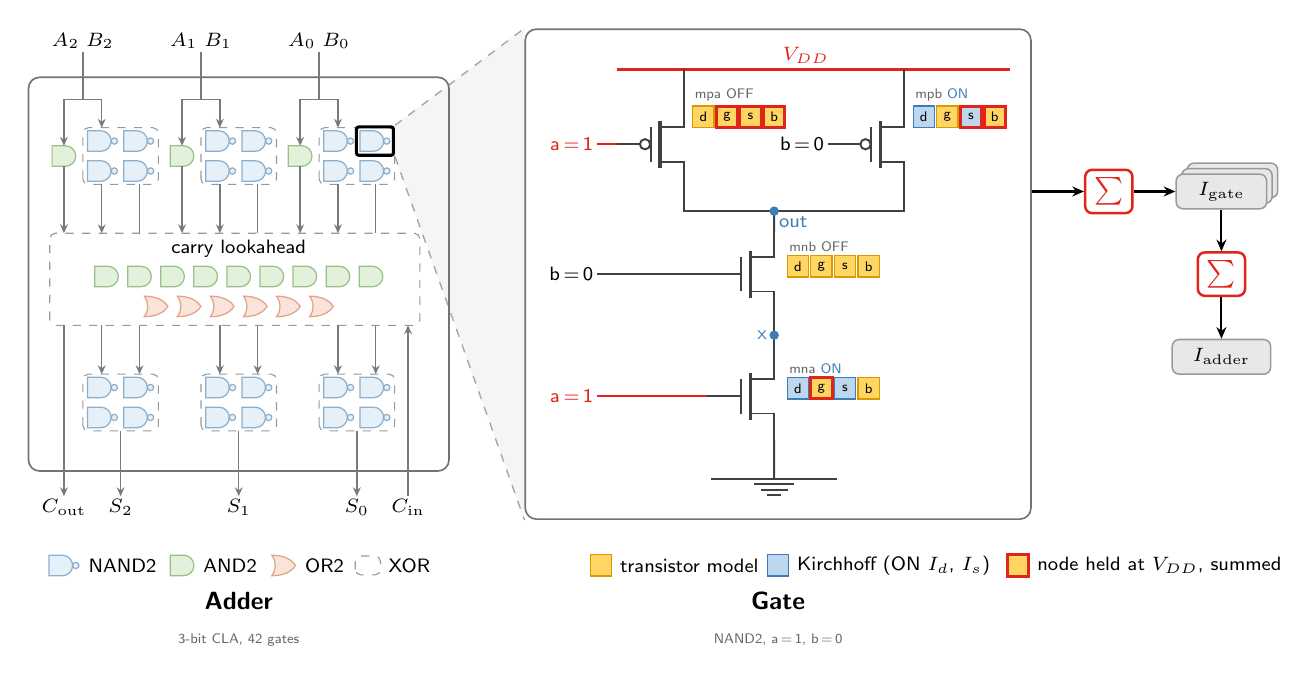
\begin{tikzpicture}

% ---------------- Adder: ports, the 42 gates of CLA_INSTANCES and the nets between the groups ----------------
% Columns are bits 2, 1, 0 at x = 0, 1.5, 3.0. Top row: P = A XOR B (four NAND2) and G = A AND B per bit.
% Middle: the carries, nine AND2 and six OR2. Bottom row: S = P XOR C per bit. The nets are drawn between
% the groups only: A and B to the XOR and the AND, P and G to the carries, P and C to the sum XOR.
\begin{scope}[shift={(0,0)}]
  \node[draw=black!55, line width=0.6pt, rounded corners=4pt, inner sep=0pt,
        fit={(-1.17,2.9) (4.17,-2.1)}] (cla) {};
  % P to the sum XOR, behind the carries.
  \foreach \cx in {0, 1.5, 3.0} {\draw[netto] ($(\cx,1.54)+(0.24,0)$) -- ($(\cx,-0.87)+(0.24,0)$);}
  % Carry lookahead.
  \draw[group, fill=white] (-0.9,-0.25) rectangle (3.8,0.92);
  \node[lab] at (1.5,0.73) {carry lookahead};
  \foreach \i in {0,...,8} {\pic at ($(1.5,0.37)+(\i*0.42-1.68,0)$) {and2};}
  \foreach \i in {0,...,5} {\pic at ($(1.5,-0.01)+(\i*0.42-1.05,0)$) {or2};}
  \foreach \bit/\cx in {2/0, 1/1.5, 0/3.0} {
    % Propagate XOR and generate AND.
    \pic at ($(\cx,1.9)+(-0.72,0)$) {and2};
    \foreach \dx/\dy in {-0.23/0.19, 0.23/0.19, -0.23/-0.19, 0.23/-0.19} {\pic at ($(\cx,1.9)+(\dx,\dy)$) {nand2};}
    \draw[group] ($(\cx,1.9)+(-0.48,-0.36)$) rectangle ($(\cx,1.9)+(0.48,0.36)$);
    % Sum XOR.
    \foreach \dx/\dy in {-0.23/0.19, 0.23/0.19, -0.23/-0.19, 0.23/-0.19} {\pic at ($(\cx,-1.23)+(\dx,\dy)$) {nand2};}
    \draw[group] ($(\cx,-1.23)+(-0.48,-0.36)$) rectangle ($(\cx,-1.23)+(0.48,0.36)$);
    % A and B to the AND and the XOR.
    \node[lab, anchor=south] (in\bit) at ($(\cx,3.22)+(-0.48,0)$) {$A_{\bit}\ B_{\bit}$};
    \draw[net] (in\bit.south) -- ($(\cx,2.62)+(-0.48,0)$);
    \draw[netto] ($(\cx,2.62)+(-0.48,0)$) -| ($(\cx,2.03)+(-0.72,0)$);
    \draw[netto] ($(\cx,2.62)+(-0.48,0)$) -| ($(\cx,2.26)+(-0.24,0)$);
    % G and P to the carries, the carry to the sum XOR, and the sum out.
    \draw[netto] ($(\cx,1.77)+(-0.72,0)$) -- ($(\cx,0.92)+(-0.72,0)$);
    \draw[netto] ($(\cx,1.54)+(-0.24,0)$) -- ($(\cx,0.92)+(-0.24,0)$);
    \draw[netto] ($(\cx,-0.25)+(-0.24,0)$) -- ($(\cx,-0.87)+(-0.24,0)$);
    \node[lab, anchor=north] (out\bit) at (\cx,-2.42) {$S_{\bit}$};
    \draw[netto] (\cx,-1.59) -- (out\bit.north);
  }
  % Carry in and carry out.
  \node[lab, anchor=north] (cin) at (3.65,-2.42) {$C_{\mathrm{in}}$};
  \draw[netto] (cin.north) -- (3.65,-0.25);
  \node[lab, anchor=north] (cout) at (-0.72,-2.42) {$C_{\mathrm{out}}$};
  \draw[netto] (-0.72,-0.25) -- (cout.north);
  % The zoomed gate: the output NAND2 of the XOR of bit 0.
  \node[draw=black, line width=1.1pt, minimum width=0.47cm, minimum height=0.36cm, inner sep=0pt,
        rounded corners=0.8pt] (pick) at (3.23,2.09) {};
  % Gate types.
  \pic at (-0.72,-3.3) {nand2};\node[lab, anchor=west] at (-0.45,-3.3) {NAND2};
  \pic at (0.78,-3.3) {and2};\node[lab, anchor=west] at (1.01,-3.3) {AND2};
  \pic at (2.07,-3.3) {or2};\node[lab, anchor=west] at (2.3,-3.3) {OR2};
  \draw[group] (2.98,-3.42) rectangle (3.3,-3.18);\node[lab, anchor=west] at (3.36,-3.3) {XOR};
  \node[title] at (1.5,-3.75) {Adder};
  \node[subtitle] at (1.5,-4.05) {3-bit CLA, 42 gates};
\end{scope}

% ---------------- NAND2 at a = 1, b = 0 ----------------
\begin{scope}[shift={(6.1,-0.55)}]
  % Rails: VDD is held high (red), ground.
  \draw[wire, draw=emph, line width=1.1pt] (0.2,3.55) -- (5.2,3.55);
  \node[lab, text=emph, anchor=south] at (2.6,3.58) {$V_{DD}$};
  \draw[wire] (1.4,-1.65) -- (3.0,-1.65);
  \foreach \i in {0,1,2} {\draw[wire] ($(1.95,-1.72)+(\i*0.08,-\i*0.07)$) -- ($(2.45,-1.72)+(-\i*0.08,-\i*0.07)$);}
  % PMOS in parallel, sources and bodies at VDD.
  \fet{mpa}{0.75}{2.6}{1}
  \fet{mpb}{3.55}{2.6}{1}
  % NMOS stack, bodies at ground: mnb (gate b) at the output, mna (gate a) at ground.
  \fet{mnb}{1.9}{0.95}{0}
  \fet{mna}{1.9}{-0.6}{0}
  \draw[wire] (mpa-top) -- (mpa-top |- 0,3.55);
  \draw[wire] (mpb-top) -- (mpb-top |- 0,3.55);
  \draw[wire] (mpa-bot) -- (1.05,1.75) -- (3.85,1.75) -- (mpb-bot);
  \draw[wire] (mnb-top) -- (2.2,1.75);
  \draw[wire] (mnb-bot) -- (mna-top);
  \draw[wire] (mna-bot) -- (2.2,-1.65);
  % Free nodes.
  \fill[kclD] (2.2,1.75) circle (0.06);
  \node[lab, text=kclD, anchor=north west] at (2.22,1.72) {out};
  \fill[kclD] (2.2,0.175) circle (0.06);
  \node[lab, text=kclD, anchor=east] at (2.15,0.175) {x};
  % Inputs: a = 1 is held high (red).
  \draw[wire, draw=emph] (mpa-g) -- (-0.05,2.6) node[lab, text=emph, anchor=east] {a\,=\,1};
  \draw[wire] (mpb-g) -- ++(-0.12,0) node[lab, anchor=east] {b\,=\,0};
  \draw[wire] (mnb-g) -- (-0.05,0.95) node[lab, anchor=east] {b\,=\,0};
  \draw[wire, draw=emph] (mna-g) -- (-0.05,-0.6) node[lab, text=emph, anchor=east] {a\,=\,1};
  % Terminal currents. Held high: VDD (PMOS sources and bodies) and a (gates of mpa and mna).
  % ON transistors (mpb, mna) take d and s from current balance, everything else from the model.
  \terms{1.3}{2.95}{m}{m,sum}{m,sum}{m,sum}{mpa}{OFF}{black!60}
  \terms{4.1}{2.95}{k}{m}{k,sum}{m,sum}{mpb}{ON}{kclD}
  \terms{2.5}{1.05}{m}{m}{m}{m}{mnb}{OFF}{black!60}
  \terms{2.5}{-0.5}{k}{m,sum}{k}{m}{mna}{ON}{kclD}
  \node[draw=black!55, line width=0.6pt, rounded corners=4pt, inner sep=6pt,
        fit={(-0.75,3.85) (5.25,-1.95)}] (gate) {};
  % Gate leakage: sum of the outlined currents. One per gate of the adder, drawn as a stack.
  \node[base, draw=emph, fill=white, line width=0.9pt, minimum width=0.6cm, minimum height=0.55cm]
    (gsum) at (6.45,2.0) {\textcolor{emph}{$\textstyle\sum$}};
  \draw[arr, draw=black] (gate.east |- gsum) -- (gsum);
  \node[tok=1.15cm] at (8.02,2.14) {};
  \node[tok=1.15cm] at (7.95,2.07) {};
  \node[tok=1.15cm] (igate) at (7.88,2.0) {$I_{\mathrm{gate}}$};
  \draw[arr, draw=black] (gsum) -- (igate);
  % Adder leakage: sum of the 42 gate leakages.
  \node[base, draw=emph, fill=white, line width=0.9pt, minimum width=0.6cm, minimum height=0.55cm]
    (asum) at (7.88,0.95) {\textcolor{emph}{$\textstyle\sum$}};
  \node[tok=1.25cm] (iadder) at (7.88,-0.1) {$I_{\mathrm{adder}}$};
  \draw[arr, draw=black] (igate) -- (asum);
  \draw[arr, draw=black] (asum) -- (iadder);
  % Legend.
  \node[m] at (0.0,-2.75) {};\node[lab, anchor=west] at (0.2,-2.75) {transistor model};
  \node[k] at (2.25,-2.75) {};\node[lab, anchor=west] at (2.45,-2.75) {Kirchhoff (ON $I_d$, $I_s$)};
  \node[m, sum] at (5.3,-2.75) {};\node[lab, anchor=west] at (5.5,-2.75) {node held at $V_{DD}$, summed};
  \node[title] at (2.25,-3.2) {Gate};
  \node[subtitle] at (2.25,-3.5) {NAND2, a\,=\,1, b\,=\,0};
\end{scope}

% Zoom from the picked gate to the gate panel.
\begin{scope}[on background layer]
  \fill[black!4] (pick.north east) -- (gate.north west) -- (gate.south west) -- (pick.south east) -- cycle;
  \draw[black!35, dashed, line width=0.5pt] (pick.north east) -- (gate.north west);
  \draw[black!35, dashed, line width=0.5pt] (pick.south east) -- (gate.south west);
\end{scope}

\end{tikzpicture}
\end{document}
